%---------------------------------------------------------------------------%
\lecture{Research Presentation}{lec_present_result}
%---------------------------------------------------------------------------%
\section{Algoritmi}
%---------------------------------------------------------------------------%
\begin{frame}[fragile]
\frametitle{Algoritmi scelti}
\begin{itemize}
    \item Supervisionato: \textbf{Decision Tree} 
    \item Non Supervisionato: \textbf{K-Means} 
\end{itemize}
\end{frame}

\begin{frame}[fragile]
\frametitle{Decision Tree}
\begin{minipage}{0.45\textwidth}
\begin{figure}
    \centering
    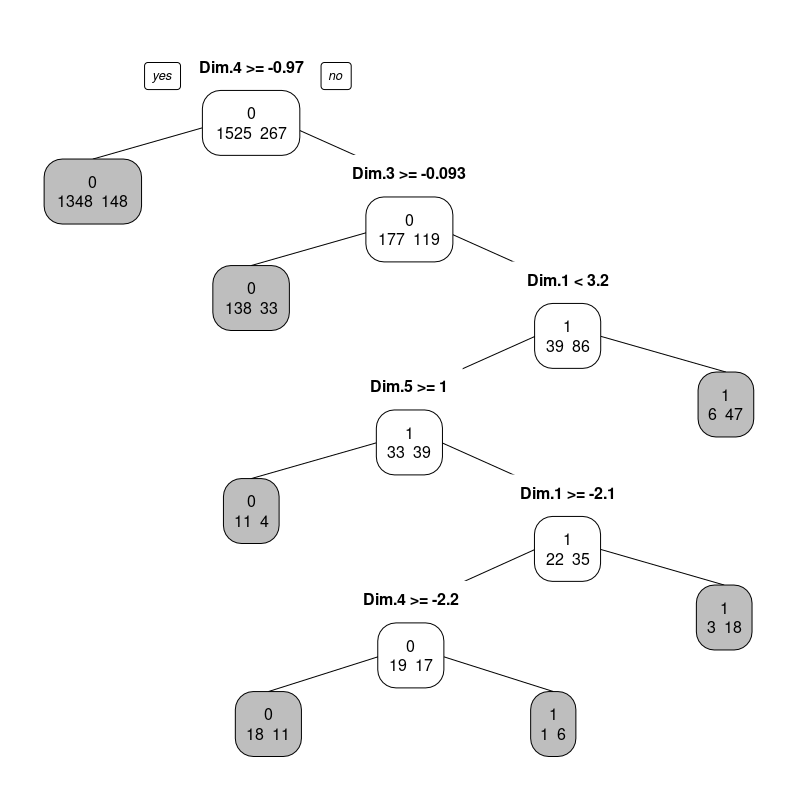
\includegraphics[width=0.8\textwidth]{Img/decision tree/D-TREE001.png}
    \caption{Decision Tree}
    \label{fig:DTREE1}
\end{figure}
\end{minipage}%
\hspace{2em}
\begin{minipage}{0.45\textwidth}

\begin{table}[h!]
\centering
\begin{tabular}{ll}
\multicolumn{2}{l}{\textbf{Positive Class:} 1} \\
\textbf{Accuracy:} 0.8348 & \textbf{Precision:} 0.1194\\
\textbf{Recall:} 0.3478 & \textbf{F-Measure:} 0.1777
\end{tabular}
\end{table}
\end{minipage}%
\end{frame}


\begin{frame}[fragile]
\frametitle{Decision Tree: Riduzione Overfitting}
\begin{minipage}{0.45\textwidth}
\begin{figure}
    \centering
    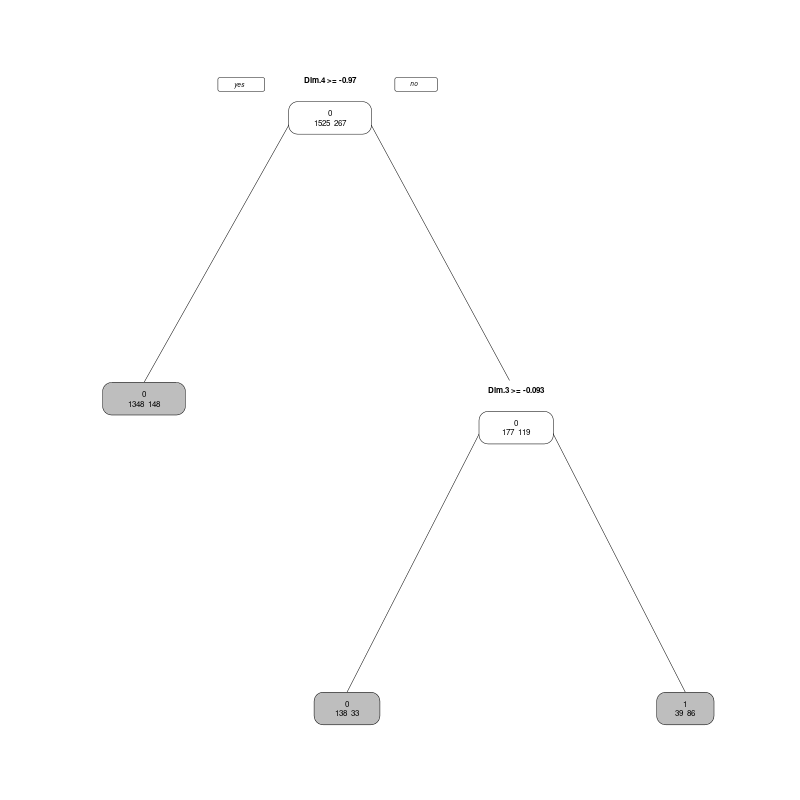
\includegraphics[width=0.8\textwidth]{Img/decision tree/D-TREE002.png}
    \caption{Decision Tree semplice}
    \label{fig:DTREE2}
\end{figure}
\end{minipage}%
\hspace{2em}
\begin{minipage}{0.45\textwidth}

\begin{table}[h!]
\centering
\begin{tabular}{ll}
\multicolumn{2}{l}{\textbf{Positive Class:} 1} \\
\textbf{Accuracy:} 0.8147 & \textbf{Precision:} 0.2777\\
\textbf{Recall:} 0.1492 & \textbf{F-Measure:} 0.1941
\end{tabular}
\end{table}

\end{minipage}%
\end{frame}

